\documentclass[a4paper,12pt]{article}
\usepackage{polski}
\usepackage[utf8]{inputenc}
\usepackage[left = 3cm, right = 3cm, top = 2cm, bottom = 2cm]{geometry}
\usepackage{enumerate}
\usepackage{amssymb}		% pakiet do symboli
\usepackage{amsmath}		% pakiet do matmy
\usepackage{enumitem}		% punktowanie (a), (b), ...
\usepackage{nopageno}		% brak numerow stron
\usepackage{graphicx}		% wstawianie obrazkow
\usepackage{float}			% wstawianie obrazkow w dowolnym miejscu
\usepackage{titling}

% nowe komendy dla wygodniejszego pisania :)
\newcommand{\subtitle}[1]{ \posttitle{ \par\end{center} \begin{center}\large#1\end{center} \vskip0.5em}}
\newcommand{\floor}[1]{\left\lfloor #1 \right\rfloor}
\newcommand{\ceil}[1]{\left\lceil #1 \right\rceil}

\begin{document}
\noindent \textbf{Lista 1, zadanie 6 - Tomasz Woszczyński}\newline

\noindent \newline \textbf{Treść:} Dany jest niemalejący ciąg $n$ liczb całkowitych dodatnich $a_1 \leq a_2 \leq \dots \leq a_n$. Wolno nam modyfikować ten ciąg za pomocą następującej operacji: wybieramy dwa elementy $a_i, a_j$, spełniające $2a_i \leq a_j$ i wykreślamy je oba z ciągu. Ułóż algorytm obliczający, ile co najwyżej elementów możemy w ten sposób usunąć.\newline

\noindent \textbf{Rozwiązanie:} Algorytm polega na podzieleniu całej tablicy na dwie tablice $L$ i $R$ o długości $\ceil{\frac{n}{2}}$ oraz $\floor{\frac{n}{2}}$, a następnie porównywaniu kolejnych elementów w następujący sposób: bierzemy pierwszy element z $L$ i usuwamy go z pierwszym elementem z $P$, który spełnia warunek $2a_i \leq a_j$. W takim przypadku zwiększamy licznik o $2$, gdyż tyle elementów jest usuwanych oraz przechodzimy do kolejnego elementu w $L$. Krok ten powtarzamy dopóki nie dojdziemy do ostatniego elementu $L$. Przedstawiony powyżej algorytm działa w czasie $O(n)$, gdyż jednokrotnie przechodzimy po całej tablicy: jednym wskaźnikiem przez $\ceil{\frac{n}{2}}$ elementów, a drugim przez $\floor{\frac{n}{2}}$ elementów. \newline

\noindent Aby rozwiązanie było optymalne, należy zawsze brać kolejne elementy z $L$ i usuwać je z pierwszymi \textbf{najmniejszymi} elementami z $R$, aby uniknąć sytuacji, w których dla np. $L=[1,2,3], R=[5,6,7]$ usuwalibyśmy pary $(1,2), (3,6)$, zamiast $(1,5), (2,6), (3,7)$. Dla optymalnego rozwiązania wykreślenie wszystkich elementów $L$ będzie oznaczało usunięcie całego ciągu, a do tego dążymy. \newline

\noindent \textbf{Dowód:} Weźmy usunięcie optymalne i załóżmy, że został pominięty jakiś element. Może to wystąpić w trzech różnych sytuacjach:
\begin{enumerate}
\item $2$ elementy w $L$: usuwając według naszego algorytmu na lewo od $a$ będziemy mieli elementy mniejsze lub równe $a$, a na prawo od $2a$ będą większe lub równe. Wtedy nasz algorytm nie pominie żadnej pary, która należy do rozwiązania optymalnego, poniżej przedstawione przykładowe sytuacje:
\begin{figure}[H]
\centering
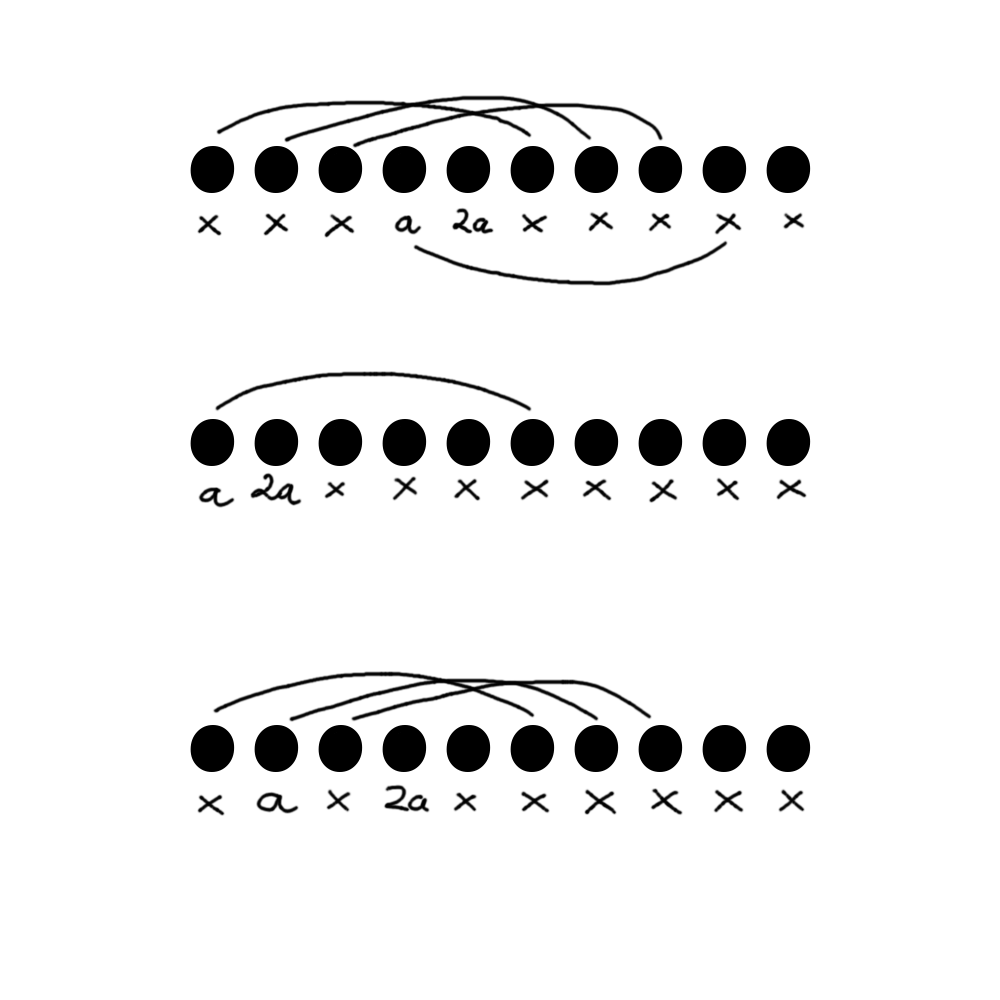
\includegraphics[width=0.65\textwidth]{2wL.png}
\end{figure}

\item $2$ elementy w $P$: usuwając elementy na pewno będziemy mogli skasować któryś z $x$ z elementem $2a$, jako że jest on dwukrotnie większy od $x$, co nam na to pozwoli, o pozostałych porównywanych wartościach nie możemy zbyt wiele powiedzieć. Przedstawia to poniżej przedstawiony rysunek:
\begin{figure}[H]
\centering
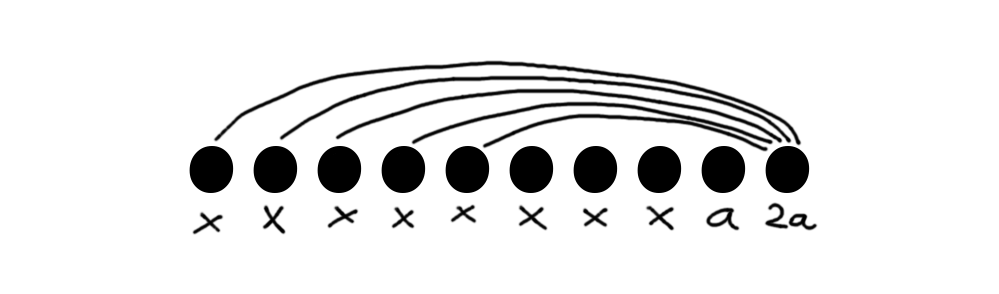
\includegraphics[width=0.65\textwidth]{2wR.png}
\end{figure}

\item po jednym elemencie w $L$ i $P$: rozpatrzmy kilka możliwych przypadków. Jeśli jakiś $x$ znajduje się na lewo od $a$ w $L$, to będzie można go wykreślić z jakąś liczbą z $P$, jako że $a \leq 2a$, ewentualnie $a$ wykreśli $2a$ (rysunek 1 i 2):
\begin{figure}[H]
\centering
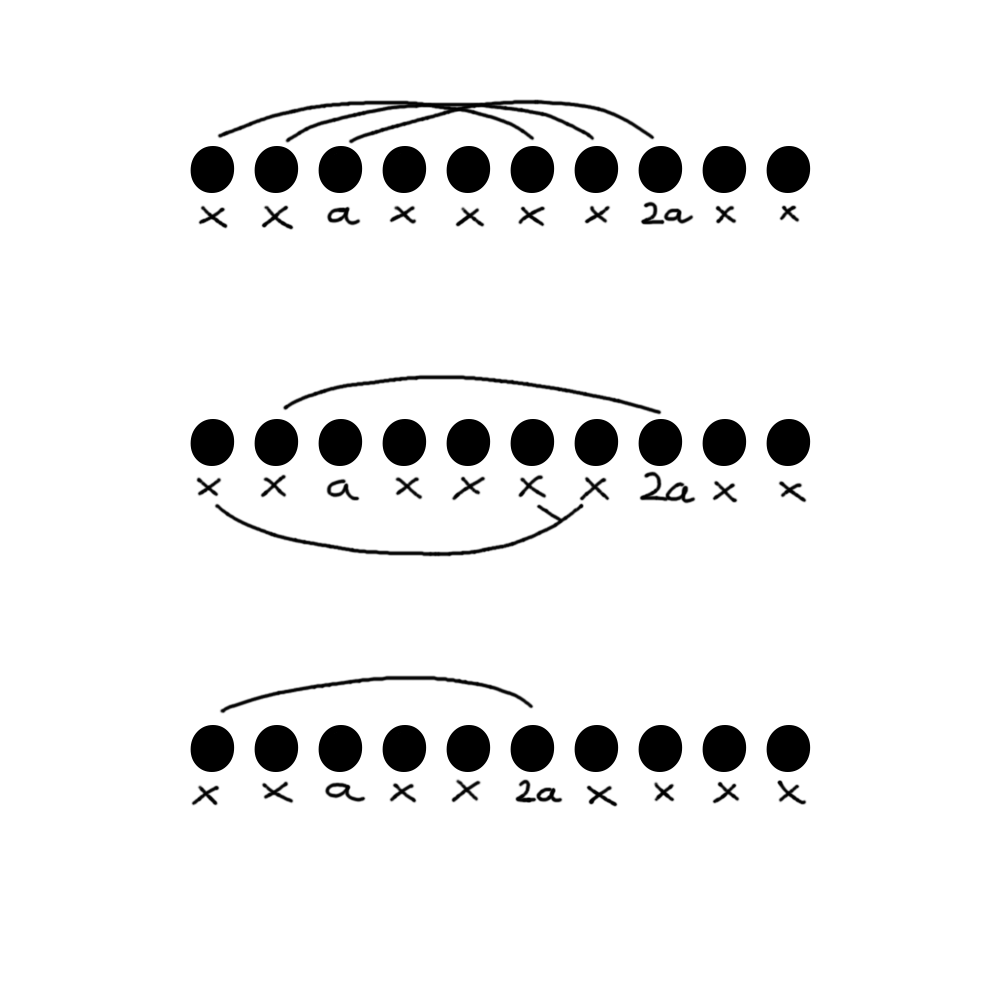
\includegraphics[width=0.65\textwidth]{LR.png}
\end{figure}
Możemy zauważyć, że w ogólnym przypadku jeśli na lewo od $a$ jest mniej liczb niż przed $2a$ w $P$, to albo wykreślimy $a$ albo $2a$. Gdy jest ich więcej, to z pewnością wykreślimy $2a$.
\end{enumerate}
Rozpatrzenie powyższych przypadków pokazuje, że algorytm jest poprawny i znajduje optymalne rozwiązanie, co kończy dowód. $\blacksquare$

\end{document}